El \textit{Banco de pruebas} fue diseñado y construido por el profesor Gerardo Arthz. Una vez fabricado se pintó la estructura, se ensambló y se cableó el motor, variador de velocidad y la térmica.

Como elementos adicionales se colocó 3 señales luminosas, potenciómetro, llave selectora de dos puntos, llave selectora de tres puntos y un pulsador. Los elementos anteriormente nombrados, fueron cableados (Figura \ref{fig:banco}(a)) hacia las borneras del variador de velocidad y se tuvo en cuenta para esto las características y funciones del bornero de control proporcionado por el manual del variador de velocidad\cite{InstaManual}. 

En la foto (Figura \ref{fig:banco}(b)) se observa el banco de pruebas del motor + variador de velocidad.

\begin{figure}[H]
	\centering
	\subfigure[]{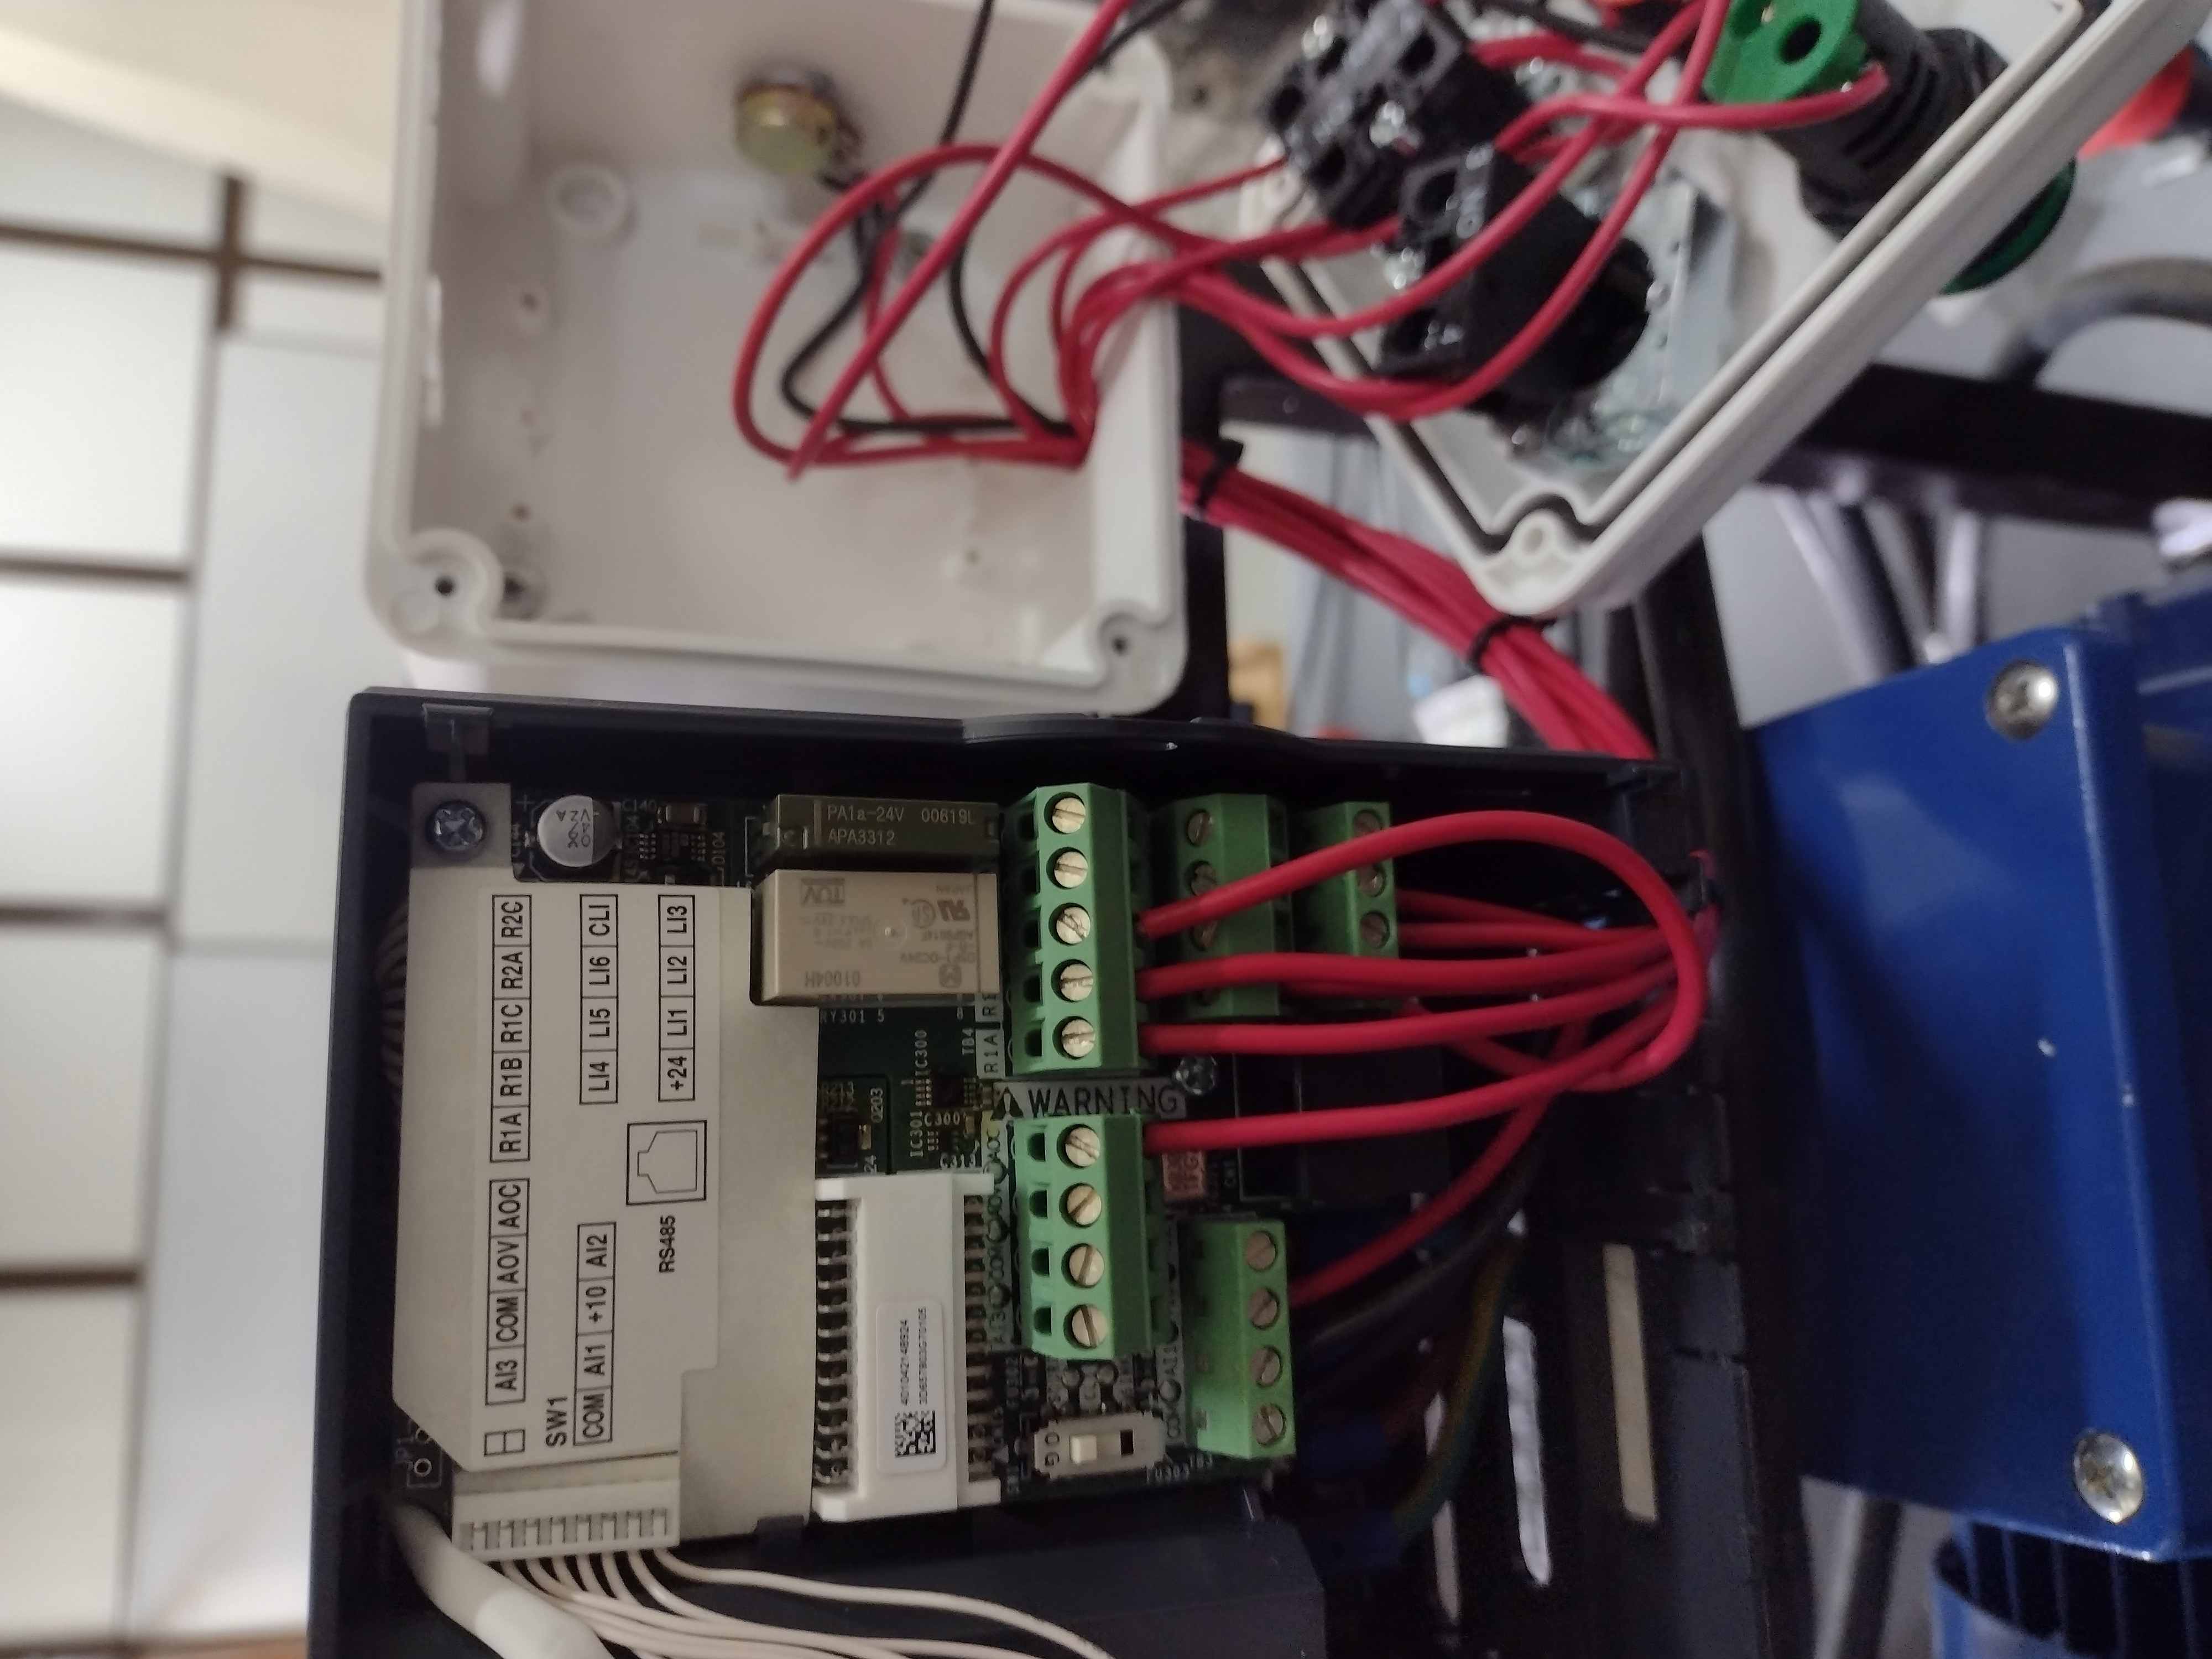
\includegraphics[angle=-90,width=60mm]{banc1 (2)}}
	\subfigure[]{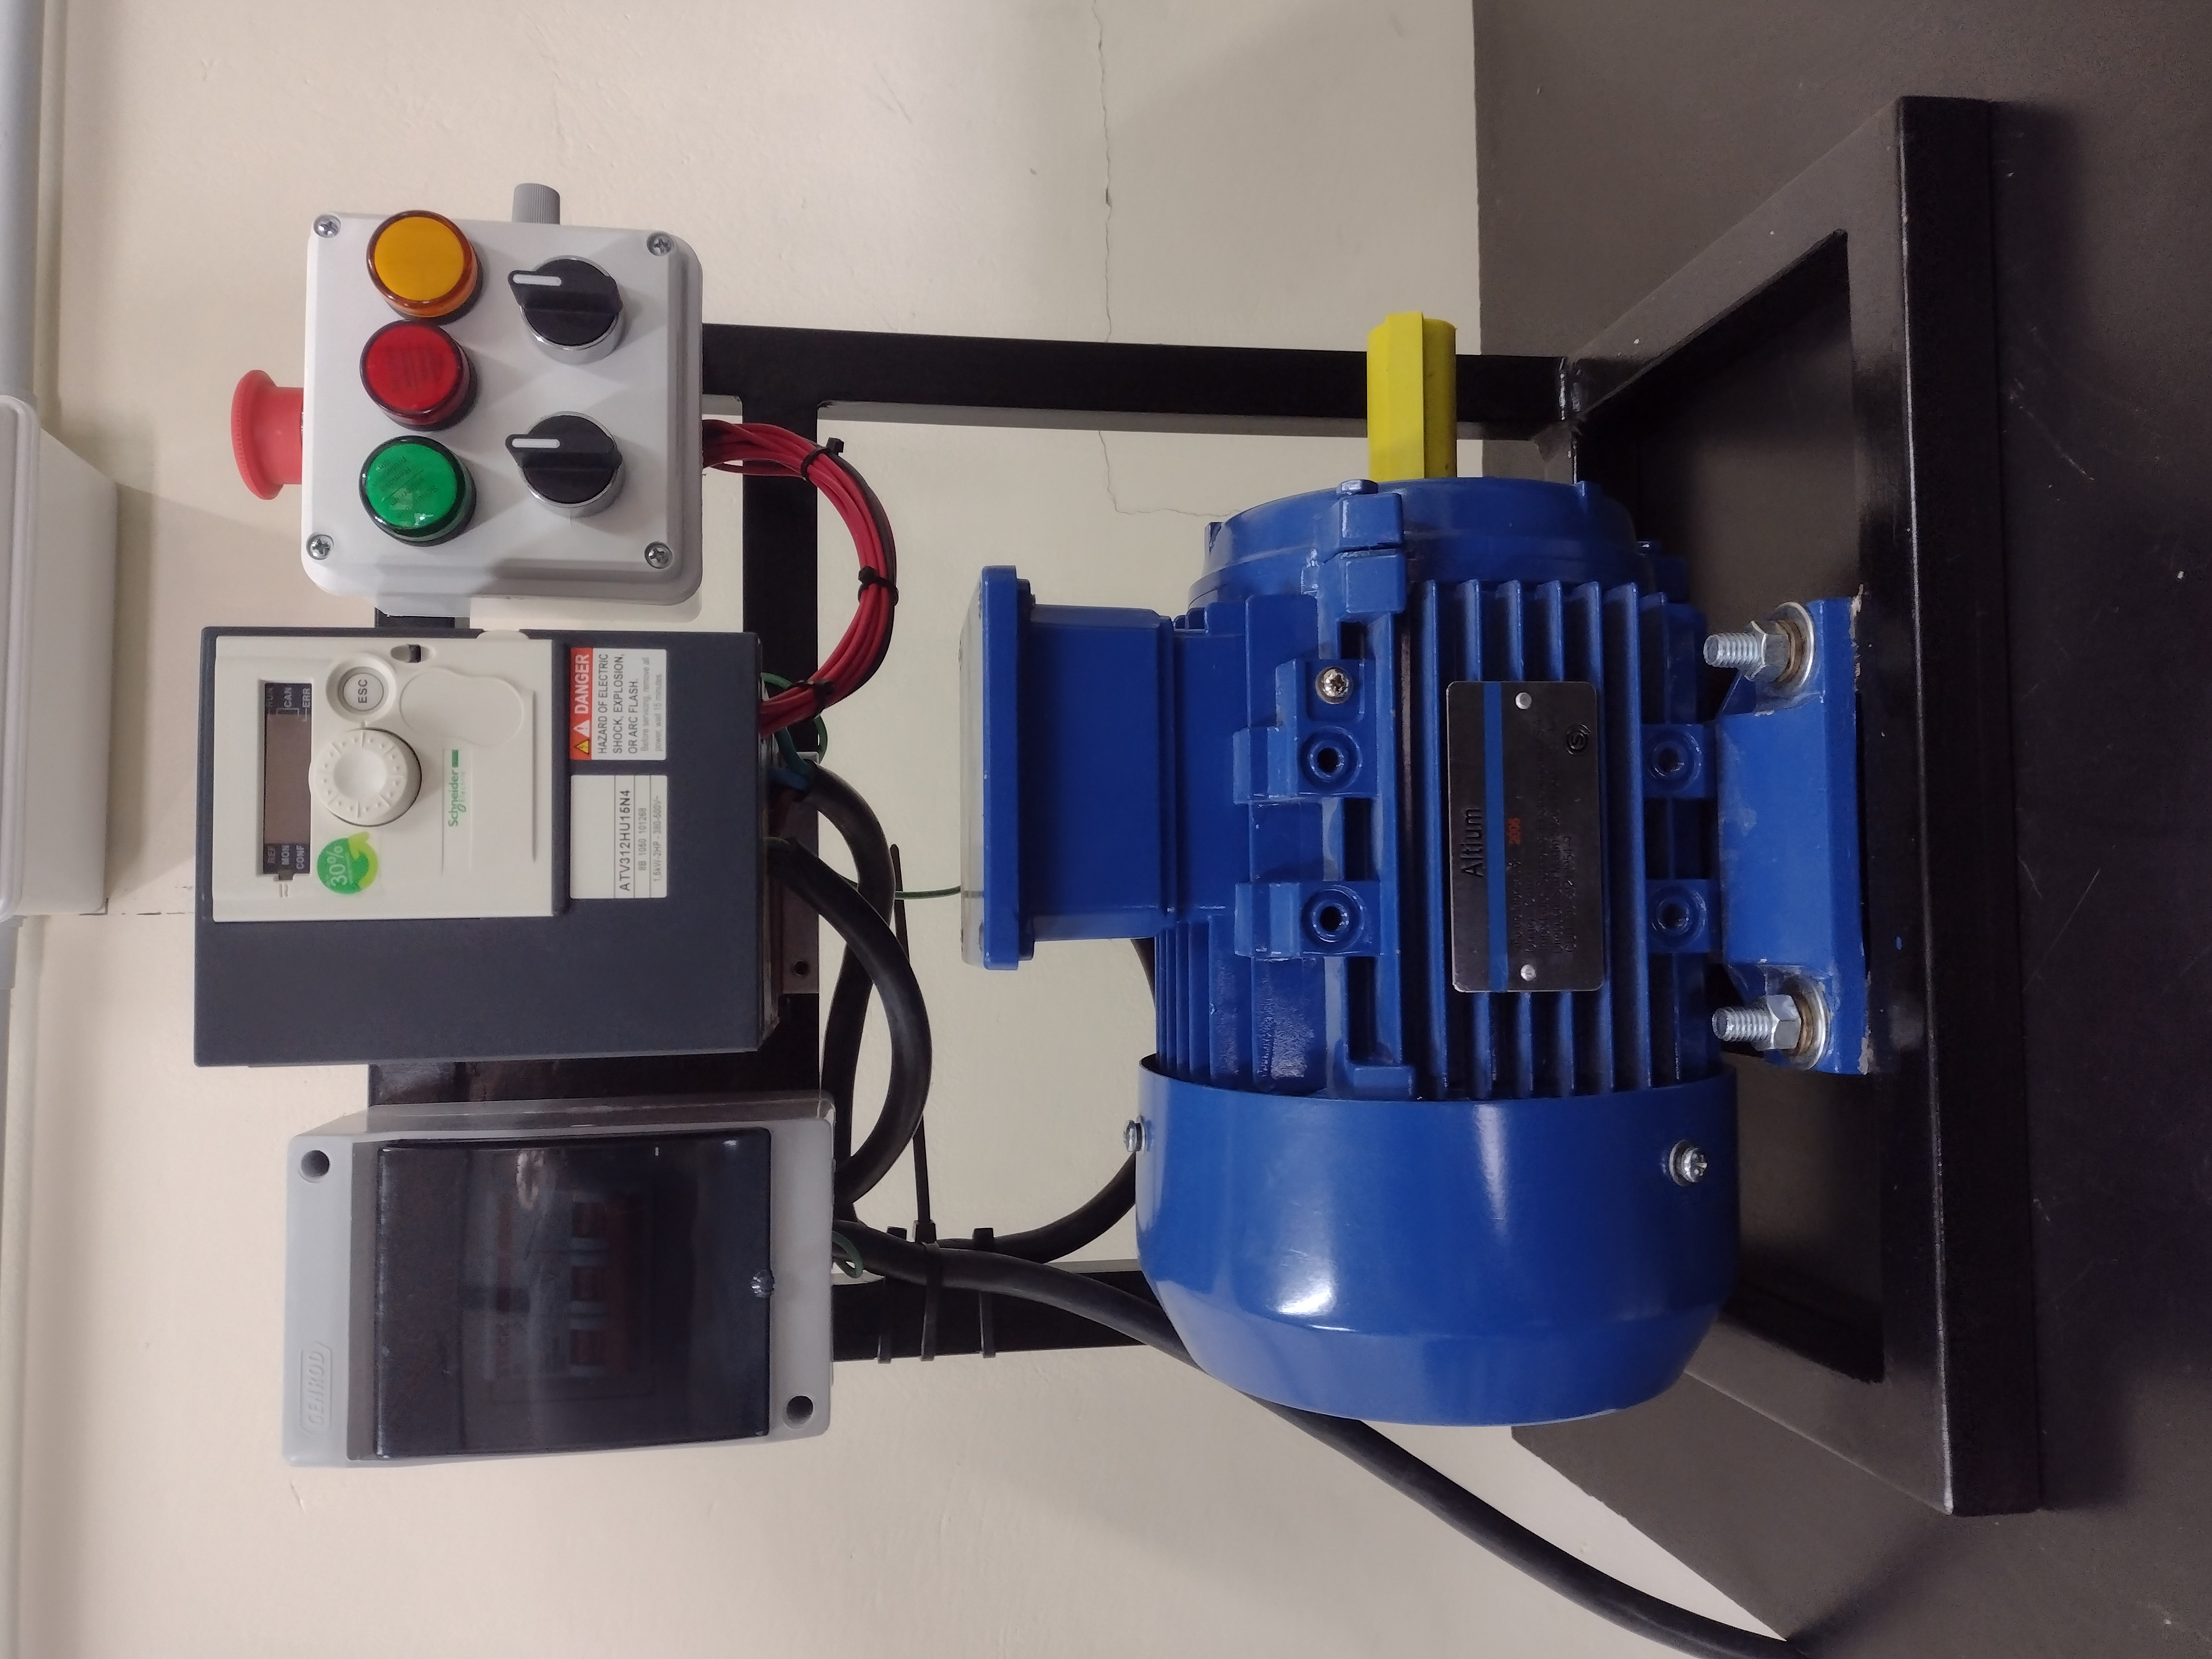
\includegraphics[angle=-90,width=60mm]{images/banc1 (1)}}
	\caption{Banco de Pruebas} \label{fig:banco}
\end{figure}



\subsection{Presupuesto}
\fcolorbox{red}{yellow}{falta lo de la bomba}
\begin{table}[H]
	\centering
	\begin{tabular}{lr|r|r|}
		\hline
		\multicolumn{1}{|c|}{\textit{\textbf{Elemento}}} & \multicolumn{1}{c|}{\textit{\textbf{Cantidad}}} & \multicolumn{1}{c|}{\textit{\textbf{Valor unitario}}} & \multicolumn{1}{c|}{\textit{\textbf{Valor total}}} \\ \hline
		\multicolumn{1}{|l|}{Antióxido 1L} & 0.33 & 798.9 & 266.3 \\ \hline
		\multicolumn{1}{|l|}{Disco corte} & 0.33 & 325.8 & 108.6 \\ \hline
		\multicolumn{1}{|l|}{Bulones 3/8 x 11/2} & 0.33 & 64.2 & 21.4 \\ \hline
		\multicolumn{1}{|l|}{Tuercas 3/8} & 0.33 & 119.5 & 39.83 \\ \hline
		\multicolumn{1}{|l|}{Arandelas 3/8} & 0.33 & 51.8 & 17.27 \\ \hline
		\multicolumn{1}{|l|}{Tubo 25x25} & 0.33 & 3140 & 1046.67 \\ \hline
		\multicolumn{1}{|l|}{Planchuela} & 0.33 & 690.06 & 230.02 \\ \hline
		\multicolumn{1}{|l|}{Caja p/termica} & 1 & 448.57 & 448.57 \\ \hline
		\multicolumn{1}{|l|}{térmica serie 3P 10A} & 1 & 1069.9 & 1069.9 \\ \hline
		\multicolumn{1}{|l|}{Señal luminosa roja 24V} & 1 & 325 & 325 \\ \hline
		\multicolumn{1}{|l|}{Señal luminosa verde 24V} & 1 & 326 & 326 \\ \hline
		\multicolumn{1}{|l|}{Señal luminosa amarilla 24V} & 1 & 326 & 326 \\ \hline
		\multicolumn{1}{|l|}{Selectora 3p} & 1 & 940.6 & 940.6 \\ \hline
		\multicolumn{1}{|l|}{Selectora 2p} & 1 & 688.5 & 688.5 \\ \hline
		\multicolumn{1}{|l|}{Pulsador emergencia} & 1 & 773.49 & 773.49 \\ \hline
		\multicolumn{1}{|l|}{Terminal presis horquilla} & 16 & 5.86 & 93.76 \\ \hline
		\multicolumn{1}{|l|}{Ficha industrial, macho 380} & 1 & 680 & 680 \\ \hline
		& \multicolumn{1}{l|}{} & \textbf{Total=    \$} & \multicolumn{1}{l|}{\textbf{7401.91}} \\ \cline{3-4} 
	\end{tabular}
\end{table}

\newpage